\documentclass{beamer}
\usetheme{metropolis}
\usepackage{graphicx}
\usepackage{subfig}
\usepackage{tcolorbox}
\title{Computer Logic and Digital Circuit Design (PHYS306/COSC330): Unit 1.3}
\author{Jordan Hanson}
\institute{Whittier College Department of Physics and Astronomy}

\begin{document}
\maketitle

\section{Summary}

\begin{frame}{Unit 1.3 Summary - Working with Binary}
\textbf{Reading: Digital Fundamentals (DF) Ch. 2 (see Moodle)}
\begin{enumerate}
\item Number representation
\item Binary conversions
\item Binary arithmetic
\item The floating-point system
\item Hexidecimals, Binary-Coded Decimals (BCD), Gray codes, and ASCII
\end{enumerate}
\textbf{Homework: exercises 1-40 Ch. 2 (DF) (two weeks)}
\end{frame}

\section{Number representation}

\begin{frame}{Number representation}
Questions:
\begin{itemize}
\item A simple question: how many students do we have in this class? \\
\item Una simple pregunta: ?`Cu\'{a}ntos estudiantes tenemos en esta clase? \\
\item Une question simple: Combien d'\'{e}tudiants est-ce que nous avons dans cette classe?
\end{itemize}
What languages do computers speak?  How can we store and transmit numbers through circuits?  (We cannot use voltage magnitudes).
\end{frame}

\begin{frame}{Number representation}
\textbf{Consider the number \alert{37}} \\ \vspace{1cm}
\begin{columns}[T]
\begin{column}{0.5\textwidth}
\centering
Numbers \\
\hrulefill
\begin{itemize}
\item 0d37
\item 0b100101
\item 0x25
\end{itemize}
\end{column}
\begin{column}{0.5\textwidth}
\centering
Expanded notation \\
\hrulefill
\begin{itemize}
\item $3\times 10^1 + 7 \times 10^0$
\item $1\times 2^5 + 1 \times 2^2 + 1 \times 2^0$
\item $2\times 16^1 + 5 \times 16^0$
\end{itemize}
\end{column}
\end{columns}
\end{frame}

\begin{frame}{Number representation}
\textbf{Consider the number \alert{412}} \\ \vspace{1cm}
\begin{columns}[T]
\begin{column}{0.5\textwidth}
\centering
Numbers \\
\hrulefill
\begin{itemize}
\item 0d412
\item 0b110011100
\item 0x100
\end{itemize}
\end{column}
\begin{column}{0.5\textwidth}
\centering
Expanded notation \\
\hrulefill
\begin{itemize}
\item $4\times 10^2 + 1\times 10^1 + 2\times 10^0$
\item $1\times 2^8 + 1\times 2^7 + 1\times 2^4 + 1\times 2^3 + 1\times 2^2$
\item $1\times 16^2$
\end{itemize}
\end{column}
\end{columns}
\end{frame}

\begin{frame}{Number representation}
\textbf{Number representations} - Digits, weights, and a common base \\ \vspace{1cm}
\begin{columns}[T]
\begin{column}{0.5\textwidth}
\centering
\begin{itemize}
\small
\item A number is written with \textbf{digits} that have \textbf{weights}.
\item A \textbf{weight} is a power of a \textbf{base}.
\item At right, the \textbf{base} is ten, and the \textbf{weights} are $10^2$, $10^1$, and $10^0$.
\item The \textbf{digits} are four, one, and two.
\item The digits cannot represent numbers larger than the base.
\end{itemize}
\end{column}
\begin{column}{0.5\textwidth}
\centering
Expanded notation \\
\hrulefill
\begin{itemize}
\item $412 = 4\times 10^2 + 1\times 10^1 + 2\times 10^0$
\end{itemize}
\end{column}
\end{columns}
\end{frame}

\begin{frame}{Number representation}
\textbf{Number representations} - (Aside) please use scientific notation, and here is why: \alert{digit minimization!} \\ \vspace{1cm}
\begin{columns}[T]
\begin{column}{0.5\textwidth}
\centering
\begin{itemize}
\small
\item Scientific notation \textbf{factors the largest weight}.
\item Results in weights that are less than one.
\item Weights that are less than one go to the right of the \textbf{decimal point}.
\item Return here with \textit{floating-point} representation.
\end{itemize}
\end{column}
\begin{column}{0.5\textwidth}
\centering
Expanded notation \\
\hrulefill
\begin{itemize}
\item $412,000,000 = 4\times 10^8 + 1\times 10^7 + 2\times 10^6 + 0\times 10^5 + 0\times 10^4 + 0\times 10^3 + 0\times 10^2 + 0\times 10^1 + 0\times 10^0$
\item $412,000,000 = 4.12 \times 10^8 = (4\times 10^0 + 1\times 10^{-1} + 2\times 10^{-2}) \times 10^8$
\end{itemize}
\end{column}
\end{columns}
\end{frame}

\begin{frame}{Number representation}
\textbf{Number representations} - (Aside) please use scientific notation, and here is why: \alert{arithmetic operations with large numbers!} \\ \vspace{1cm}
\begin{enumerate}
\item $4200 \times 4200 = (4.2 \times 10^{3})^2 = (4.2)^2 \times 10^6 \approx 16 \times 10^6$
\item $\approx 17.6 \times 10^6$ if you account for the $0.2$ ...
\end{enumerate}
\hrulefill
\begin{enumerate}
\item $4000/3000 = 4 \times 10^{3} \times \frac{1}{3} \times 10^{-3} = \frac{4}{3}$
\item $\frac{4}{3} \approx 1.33$
\end{enumerate}
\end{frame}

\begin{frame}{Number representation}
Expand the following numbers to expanded decimal notation:
\begin{itemize}
\item -10.432
\item 800,000,144
\end{itemize}
Expand the following numbers to expanded binary notation:
\begin{itemize}
\item 10011010
\item 11110000
\end{itemize}
Convert the following decimal numbers to binary notation:
\begin{itemize}
\item 260
\item 560
\end{itemize}
\textbf{Volunteer to board?} - Key is explaining how you did the binary conversions
\end{frame}

\section{Binary Conversion}

\begin{frame}{Binary Conversion}
How did you do the conversions to binary?  Is there a systematic what to do this? \\
\begin{itemize}
\item \textit{Successive Approximation} - like a number puzzle (\textit{Sum of Weights Method})
\item \textit{Successive Division Method} - Example of an algorithm
\end{itemize}
\hrulefill \\ \vspace{0.5cm}
\textit{Successive approximation} technique (does this remind you of doing division in your head?)
$260$...$2^8 = 256$.  Now we need four more...$4 = 2^2$.  So $2^8 + 2^2 = 0b10000100$ \\ \vspace{0.5cm}
What is 328 divided by 3?  Ok try 100 because three times one hundred is close...
\end{frame}

\begin{frame}{Binary Conversion}
\textit{Successive Division Method} \\ \vspace{0.5cm} \hrulefill \\
$0d412 = 0b110011100 = 2^8 + 2^7 + 2^4 + 2^3 + 2^2$ \\
Algorithm:
\begin{enumerate}
\item Divide the decimal number by 2, and write down the remainder.  This is the \textit{least-significant bit} or LSB.
\item Keep dividing and recording the remainders in order, until you reach a dividend of 1.
\item $1/2 = 0 r 1$, so the \textit{most-significant bit}, or MSB, is always 1.
\end{enumerate}
Convert 412 to binary using the successive division method.
\end{frame}

\begin{frame}{Binary Conversion}
Convert the numbers at right to binary. \\ \vspace{1cm}
\begin{columns}[T]
\begin{column}{0.5\textwidth}
\begin{itemize}
\item $2^0 = 1$
\item $2^1 = 2$
\item $2^2 = 4$
\item $2^3 = 8$
\item $2^4 = 16$
\item $2^5 = 32$
\item $2^6 = 64$
\item $2^7 = 128$
\end{itemize}
\end{column}
\begin{column}{0.5\textwidth}
\begin{enumerate}
\item 93
\item 189
\item 270
\end{enumerate}
\textit{Note: how many bits do you need for that last one?}  For binary, show that the highest representable number with $n$ bits is $2^n-1$.
\end{column}
\end{columns}
\end{frame}

\begin{frame}{Binary Conversion}
In decimal notation, we represent numbers $\in [0-1]$ with digits to the right of the \textit{decimal point.} \\ \vspace{0.5cm}
In expanded notation: \\
$42.42 = 4\times 10^{1} + 2\times 10^{0} ~~ . ~~ 4\times 10^{-1} + 2\times 10^{-2}$ \\ \vspace{0.5cm}
We have a similar notation in other number systems: \\
$101.11 = 2^2 + 2^0 ~~ . ~~ 2^{-1} + 2^{-2}$
\end{frame}

\begin{frame}{Binary Conversion}
\textit{Successive Multiplication Method} \\ \vspace{0.5cm} \hrulefill \\
$0d0.48 = 0b0.011110101 = 2^{-2}+2^{-3}+2^{-4}+2^{-5}+2^{-7}+2^{-9}$ \\
Algorithm:
\begin{enumerate}
\item Multiply the decimal fraction by 2, and write down the \textit{carry} (the 1 to the left of the decimal point, else 0).  This is the \textit{most-significant bit} or MSB.
\item Keep multiplying and recording the carries in order, to the desired precision.
\item Watch for repeating patterns.
\end{enumerate}
Convert 0.48 to binary using the successive multiplication method until you identify a repeating pattern.
\end{frame}

\section{Binary Arithmetic}

\begin{frame}{Binary Arithmetic}
Binary arithmetic, like decimal arithmetic, relies upon \textit{carries} and \textit{borrows}.  For example in decimal: \\ \vspace{0.5cm}
\begin{itemize}
\item $8+7 = 5 c 1 = 15$
\item $3+4 = 7 c 0 = 7$
\item $8-2 = 6 b 0 = 6$
\item $10-5 = (0 b 10) - 5 = 5$
\item $13-7 = (0 b 10) - 4 = 6$ 
\end{itemize}
\end{frame}

\begin{frame}{Binary Arithmetic}
In binary there are limited combinations, so we may form a set of addition and subtraction rules that describe all possibilities: \\ \vspace{0.5cm}
\hrulefill
\begin{columns}[T]
\begin{column}{0.5\textwidth}
\begin{itemize}
\item $0+0=0$
\item $1+0=1$
\item $0+1=1$
\item $1+1 = 0 c 1$
\end{itemize}
\end{column}
\begin{column}{0.5\textwidth}
\begin{itemize}
\item $0-0=0$
\item $1-0=1$
\item $0-1=0b1$
\item $1-1 = 0$
\end{itemize}
\end{column}
\end{columns}
\tiny
In the fourth rule for the addition set, the carry works the same way as a decimal carry: we add that $1$ to the digit corresponding to the next power of 2.  Similarly, in the third rule of the subtraction set, we subtract the $1$ on the left side of the equation from a $1$ from the digit corresponding to the next highest power of 2 available.
\end{frame}

\begin{frame}{Binary Arithmetic}
Complete the following additions and subtractions: \\ \vspace{0.5cm}
\hrulefill
\begin{columns}[T]
\begin{column}{0.5\textwidth}
\begin{itemize}
\item $10+11$
\item $111+1$
\item $111+111$
\item $1010+101$
\end{itemize}
\end{column}
\begin{column}{0.5\textwidth}
\begin{itemize}
\item $10-11$
\item $111-1$
\item $111-111$
\item $1010-101$
\end{itemize}
\end{column}
\end{columns}
\end{frame}

\begin{frame}{Binary Arithmetic}
Binary multiplication stems from another set of rules: \\ \vspace{0.5cm}
\hrulefill
\begin{columns}[T]
\begin{column}{0.5\textwidth}
\begin{itemize}
\item $0\times 0=0$
\item $1\times 0=0$
\item $0\times 1=0$
\item $1\times 1=1$
\end{itemize}
\end{column}
\begin{column}{0.5\textwidth}
\small
Binary division is exactly the same as decimal long division.  Let's work these examples on the board:
\begin{itemize}
\item 145/12
\item 1101/101
\item 45/3
\item 111/10
\end{itemize}
\end{column}
\end{columns}
\small
Of what logic operation does binary multiplication remind you?
\end{frame}

\begin{frame}{Binary Arithmetic}
We need a few tools to improve our arithmetic techniques in order to install these functions into circuits.  Consider two actions:
\begin{itemize}
\item NOT to the bit sequence of a number: \textbf{\alert{1's compliment}}
\item Add 1 to the 1's compliment: \textbf{\alert{2's compliment}}
\end{itemize}
\end{frame}

\begin{frame}{Binary Arithmetic}
Logical operator representation of these actions for 8-bits: \\ \vspace{0.5cm}
\hrulefill
\begin{columns}[T]
\begin{column}{0.5\textwidth}
\begin{figure}
\centering
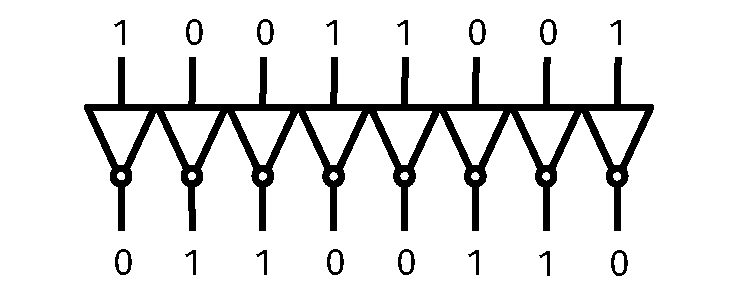
\includegraphics[width=\textwidth]{figures/1Compliment.pdf}
\caption{\label{fig:1comp} Representation of 1's compliment.}
\end{figure}
\end{column}
\begin{column}{0.5\textwidth}
\begin{figure}
\centering
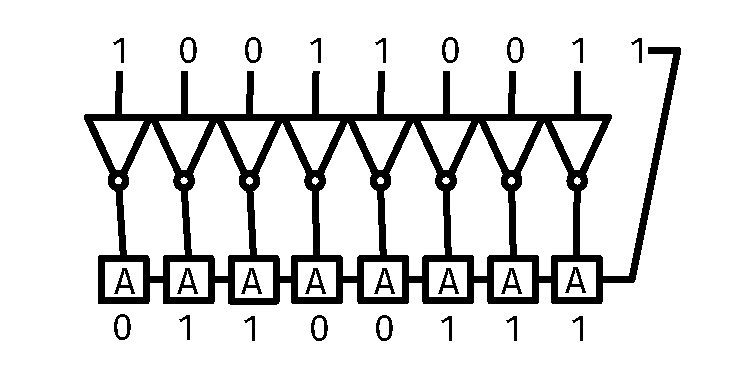
\includegraphics[width=\textwidth]{figures/2Compliment.pdf}
\caption{\label{fig:2comp} Representation of 2's compliment.}
\end{figure}
\end{column}
\end{columns}
\end{frame}

\begin{frame}{Binary Arithmetic}
Exercises, and a realization for the purpose of 2's compliment. \\ \vspace{0.5cm}
\hrulefill
\begin{columns}[T]
\begin{column}{0.33\textwidth}
Take the 1's compliment of the right-hand number, and complete the addition:
\begin{itemize}
\item $111+(000)$
\item $111+(111)$
\end{itemize}
\end{column}
\begin{column}{0.33\textwidth}
Take the 2's compliment of the right-hand number, and complete the addition:
\begin{itemize}
\item $111+(000)$
\item $111+(111)$
\end{itemize}
\end{column}
\begin{column}{0.33\textwidth}
Same, \alert{but drop the MSB}:
\begin{itemize}
\item $1010+(1010)$
\item $1100+(1100)$
\end{itemize}
\end{column}
\end{columns}
\vspace{0.5cm}
\small
For what purpose are we going to use the 2's compliment?
\end{frame}

\begin{frame}{Binary Arithmetic}
The answer: representing negative numbers.  For \textit{2's compliment form signed binary numbers, the MSB is the \textbf{sign bit}}.  To convert to decimal, \alert{give the MSB a negative weight}: \\ \vspace{0.5cm}
Example: $10101010$ \\ 
This is a negative number because the MSB is a $1$.  Converting in expanded form: $-2^7+2^5+2^3+2^1 = -128+32+8+2 = -86$.
\end{frame}

\begin{frame}{Binary Arithmetic}
Consider the effect on the maximum \textit{range} of binary numbers after sacrificing the MSB to flag numbers less than zero.  For 8-bits unsigned numbers, the range is [0-255]: \\ \vspace{0.5cm}
\begin{table}
\small
\centering
\begin{tabular}{c c c c}
$n$-bits & 8 & 16 \\
Lowest unsigned & 0 & 0 \\
Highest unsigned & 255 & 65535 \\
Lowest signed & -128 & -32768 \\
Highest signed & 127 & 32767
\end{tabular}
\caption{\label{tab:ranges} The ranges of unsigned and signed numbers using $n$ digits.}
\end{table}
\small
By changing the role of the MSB, we are not reducing the \textit{range} of numbers, just its \textit{location}.  Related to \textit{conservation of information...}
\end{frame}

\section{Conclusion}

\begin{frame}{Unit 1.3 Summary - Working with Binary}
\textbf{Reading: Digital Fundamentals (DF) Ch. 2 (see Moodle)}
\begin{enumerate}
\item Number representation
\item Binary conversions
\item Binary arithmetic
\item The floating-point system
\item Hexidecimals, Binary-Coded Decimals (BCD), Gray codes, and ASCII
\end{enumerate}
\textbf{Homework: exercises 1-40 Ch. 2 (DF) (two weeks)}
\end{frame}

\end{document}
